\subsubsection{Mining on manifolds}\label{subsec:mining_manifolds}


% sparse usage of hard pairs inspired by SVMs

% purpose
According to \citet{mining_manifolds_2018}, the initial representation of the data is obtained by e.g. a pre-trained \ac{cnn}.
Hard pair mining is performed in order to re-train the network.

% idea of positive and negative samples
For re-training, a combination of different definitions of proximity induces mining 
for hard positives and negatives as displayed in \autoref{fig:mining_manifolds_vis}.
Given an anchor, the neighbours on the same manifold which are not neighbours in terms of 
Euclidean proximity are considered hard positive samples.
These positive samples should be embedded closer to the anchor in the Euclidean space.
Hard negative samples, on the other hand, are neighbours in Euclidean space, 
but on different manifolds.
These samples should be embedded further away from the anchor in the Euclidean space.
%The hard samples are mined from an unordered set of \textit{relevant} samples.

% different neighbourhoods & hard samples
The authors define the $k$ nearest Euclidean neighbour $NN^e_k$ and 
the $k$ nearest manifold neighbour $NN^m_k$.
The hard positives are defined as $NN^m_k \textbackslash NN^e_k$. 
The pool $NN^m_k$ is ordered by descending manifold similarity to the anchor
to ensure that high-confidence samples are chosen first.
$k$ controls the diversity of the hard positives.
The larger $k$ is, the more diverse, i.e. hard, the hard positives are. 
The pool of hard negatives is defined as $NN^e_k \textbackslash NN^m_k$.
$NN^e_k$ is ordered by descending Euclidean distance to the anchor to keep the hardest samples.

% visualization of hard samples
\begin{figure}[!htb]% h = here, t = top, b = bottom, p = page of floats
    \centering
    \subfloat[\centering $k$ nearest Euclidean neighbour $NN^e_k$ (orange).]
    {{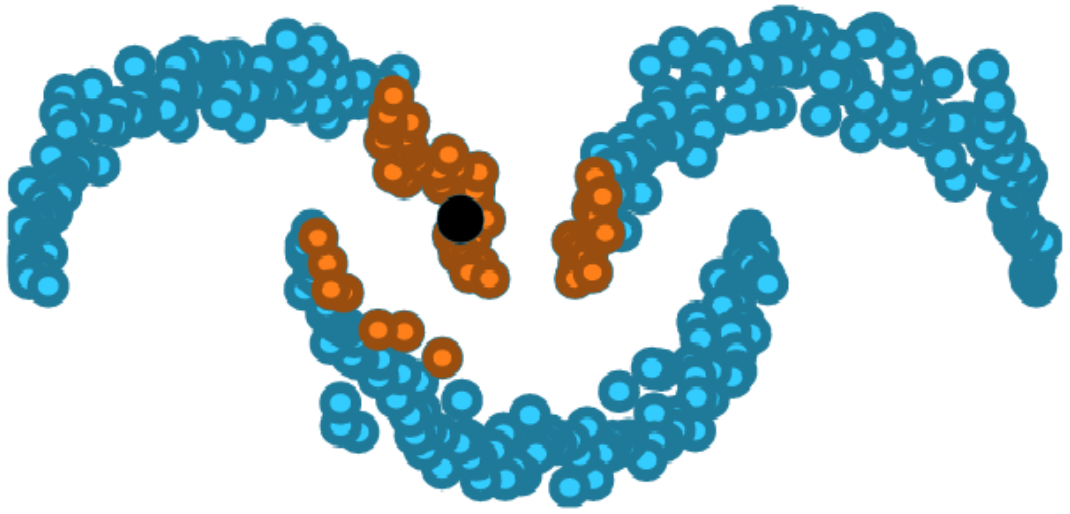
\includegraphics[width=5cm]{images/euclidean_NN.png} }}%
    \qquad
    \subfloat[\centering $k$ nearest manifold neighbour $NN^m_k$ (purple).]
    {{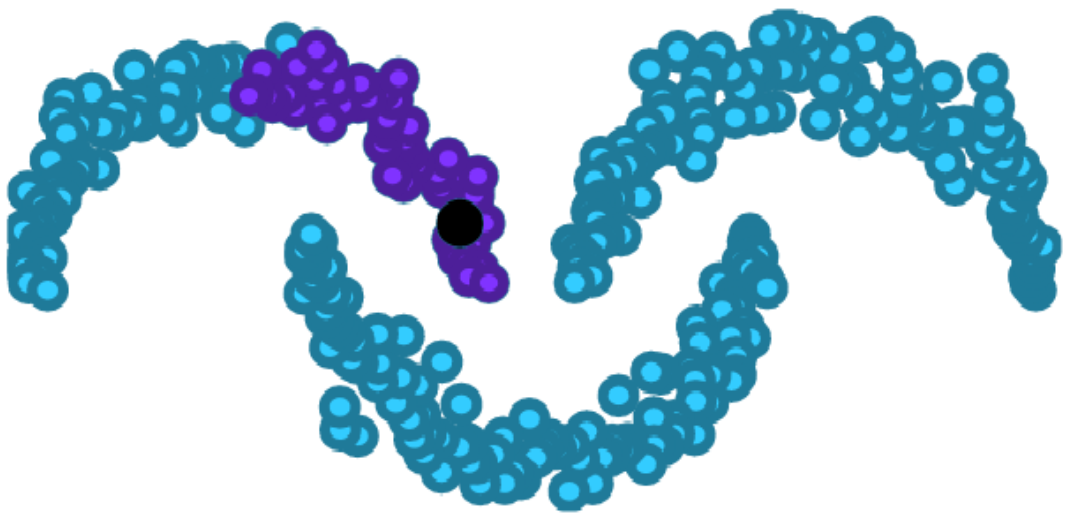
\includegraphics[width=5cm]{images/manifold_NN.png} }}%
    \qquad
    \subfloat[\centering Hard positives $NN^m_k \textbackslash NN^e_k$(green).]
    {{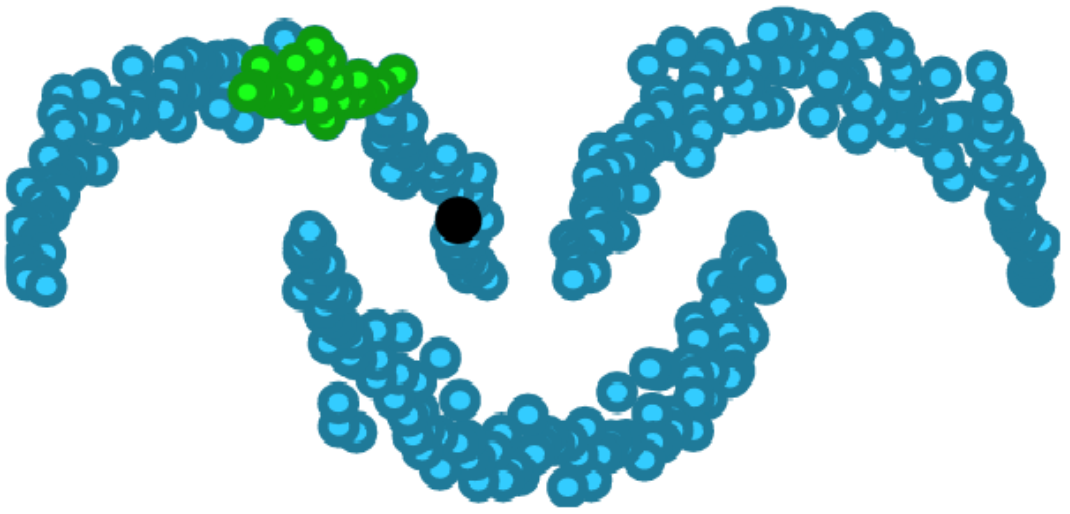
\includegraphics[width=5cm]{images/hard_positives_manifold.png} }}%
    \qquad
    \subfloat[\centering Hard negatives $NN^e_k \textbackslash NN^m_k$(red).]
    {{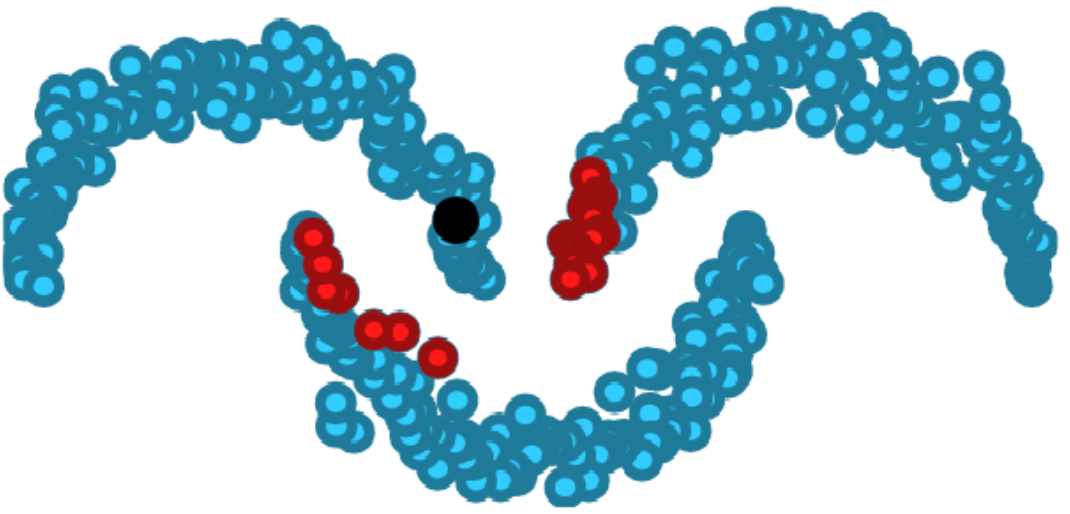
\includegraphics[width=5cm]{images/hard_negatives_euclidean.png} }}%

    \caption{Visualization of different proximity definitions and 
    the hard negatives/positives from \citet{mining_manifolds_2018}.
    The anchor is the black point.}%
    \label{fig:mining_manifolds_vis}%
\end{figure}


% manifolds via random walk n nearest neighbour graph
\citet{mining_manifolds_2018} propose a method where the manifold is estimated by mode-seeking, i.e. a random walk process, 
on the Euclidean nearest neighbour graph induced by the Euclidean similarity function $s_e$.
The graph is undirected, weighted and represented by a sparse symmetric adjacency matrix.
The adjacency matrix consists of the reciprocal $k$ nearest neighbours of each sample. 
To reduce the negative impact of outliers, only reciprocal nearest neighbours are incorporated \citet{diffusion_2017,mining_manifolds_2018,fast_2018}.
The weighted adjacency matrix entries $a_{ij}$ defined in \eqref{eq:mining_manifolds_adjacency_matrix} from \citet{mining_manifolds_2018} 
are calculated via the Euclidean distance between the samples if both nodes are in each other's nearest neighbourhood.
Diagonal entries are set to zero \citet{mining_manifolds_2018,fast_2018}.
%They admit that assessing the manifold similarity poses additional computational and memory requirements.
The manifold is computed once at the beginning \citet{mining_manifolds_2018}.

\begin{equation}
    a_{ij} = \begin{cases}
        s_e(y_i,y_j), & \text{if } y_i \in NN^e_k(y_j)\wedge y_j \in NN^e_k(y_i)\\
        0, & \text{otherwise}\\
      \end{cases}     
    \label{eq:mining_manifolds_adjacency_matrix}
\end{equation}


% mode seeking
% The manifold representation is obtained via mode-seeking as described in \citet{mode_seeking_2012}.
% The nearest neighbour network consists of samples as nodes and is weighted by the Euclidean distance 
% if both samples are in each other's $k$ nearest neighbourhood \citet{mode_seeking_2012,mining_manifolds_2018}.

% authority modes
While traditional mode-seeking relies on metric features, such as distances, mode-seeking on graphs 
uses the concept of random walks instead \citet{mode_seeking_2012}.
A random walk, i.e. a linear combination of the identity matrix and a scaled version of the adjacency matrix, is simulated multiple times on the graph.
\citet{mode_seeking_2012} define the so-called authority modes on a graph 
as the most frequently visited nodes by random walks among their local neighbours.
They correspond to the local maxima of the underlying probability distribution of random walks over the graph.
% selection of anchors
Since the anchors should be diverse and relevant, they are chosen to be the authority modes \citet{mining_manifolds_2018}.

% authority score
Inspired by PageRank, the possibility of random jumps is included in order to ensure convergence to a stationary distribution. 
The probability of visiting a node is denoted by the authority score $\pi$ 
which is defined in \eqref{eq:authority_score} from \citet{mode_seeking_2012} 
where $p(i,j)$ are the entries of the Markov transition matrix $P$.
$\pi(j)$ takes into account the probability of visiting a node $j$ from a node $i$ and 
the probability of a random jump from one of the nodes chosen uniformly at random.
\citet{mode_seeking_2012} set $\alpha$ to $0.9$. 
The authority score $\pi$ can be computed by, for instance, the power method \citet{mode_seeking_2012,PageRank_2004}.

\begin{equation}
    \pi(j) = \alpha \sum_{i \in \mathcal{V}}^{}  \pi(i)p(i,j) + (1-\alpha)\frac{1}{N} , \text{ where } p(i,j) = \frac{a_{ij} }{\sum_{k \in \mathcal{V}}^{}a_{ik} } 
    \label{eq:authority_score}
\end{equation}

% local neighbours on the manifold: node relevancy 
\citet{mode_seeking_2012} define node relevancy $\Psi(s,t)$ via \eqref{eq:node_relevancy} where $d(s)$ denotes the out-degree of a node.
To incorporate the reachability of a node, the probability of reaching node $t$ from node $s$ in $k$ steps $p_k(s,t)$ is 
defined via the $k_{th}$ power of the Markov transition matrix $P$.
To support similar authority scores between neighbouring nodes, the exponential term including a weighting factor $\gamma$ is included.
$\Psi(s,t)$ is not symmetric and depends on the random walk step $k$.
The authors propose to use the node relevancy $\Psi(s,t)$ for a node $s$ to determine the manifold neighbours $N_\varepsilon^m(s)$ for $s$ 
via the usage of a threshold $\varepsilon$: 
$N_\varepsilon^m(s) =  \left\{ t \in \mathcal{V} | \Psi(s,t) > \varepsilon \right\} \cup \left\{ s \right\}$ \citet{mode_seeking_2012}.

\begin{equation}
    \Psi(s,t) = d(s) p_k(s,t) \exp(-\gamma \left\{  \pi(t) - \pi(s)  \right\}^2)\text{, where } d(s) = \sum_{j\in \mathcal{V}}^{}a_{sj}
    \label{eq:node_relevancy}
\end{equation}

% AAS
They propose the \ac{aas} as a nonparametric estimator of the authority modes.
A node $s$ is shifted to node $\mathcal{A}(s)$ calculated in \eqref{eq:authority_ascent_shift}. 
This formula chooses the local neighbour $t$ of $s$ that maximizes the difference of the authority scores $\pi$.
The authors argue that the \ac{aas} is finite and converges since the graph is finite.
When \ac{aas} is completed, manifolds are represented as clusters.

\begin{equation}
    \mathcal{A}(s) = \underset{t \in \mathcal{N_\varepsilon}(s)}{\text{argmax}} \left\{ p_k(s,t)\left[ \pi(t)-\pi(s) \right] \right\}
    \label{eq:authority_ascent_shift}
\end{equation}

% inlier and outlier
% Inliers on the manifold reside in large clusters while outliers are isolated in small groups since they do not have enough relevancy with inliers \citet{mode_seeking_2012}.
% Hence, outlier clusters can be identified by low sums of authority values.


% loss functions
The authors propose multiple loss functions to train the model.
They, for instance, apply the contrastive loss $l_c(x^r, x^+, x^-)= \left\| x^r - x^+ \right\|^2 + \left[ m - \left\| x^r - x^- \right\| \right]^2$, 
the triplet loss $l_t(x^r, x^+, x^-)= \left[ m +  \left\| x^r - x^+ \right\| ^2 - \left\| x^r - x^- \right\| \right]^2$, 
and weighted versions of both contrastive and triplet loss, where the loss is multiplied by the manifold similarity of anchor and positive sample \citet{mining_manifolds_2018}.
$m$ is a margin parameter and $x^r$ is the representation of the anchor.

% examples
Resulting hard positives and negatives are displayed in \autoref{fig:manifold_mining_qualitative_analysis} and \autoref{fig:manifold_mining_examples}.

\begin{figure}[!htb] % h = here, t = top, b = bottom, p = page of floats
    \centering
    \includegraphics[width=360pt]{images/mining_manifold_qualitative_analysis.png}
    \caption{Illustration of CUB200-2011 from \citet{mining_manifolds_2018}.
    The anchor is denoted $x^r$.
    A selection of hard positives from $P^+(x^r)$ is compared to the 
    baseline approach by sampling from the closest neighbours to $x^r$ in 
    terms of Euclidean distance.
    Analogously, a selection of hard negatives from $P^-(x^r)$ 
    is compared to the baseline $X \textbackslash NN^e_3$, 
    i.e. sampling from the set that contains all samples but the three closest ones in 
    terms of Euclidean distance.
    The borders of the images denote the ground-truth class, i.e. if bird species is the same.
    Green borders mean that the image belongs to the same class as the anchor,
    whereas red denotes different class images.
    It becomes apparent that the sampled hard positives consist of fewer false positives 
    as the baseline.
    }
    \label{fig:manifold_mining_qualitative_analysis}
\end{figure}

\begin{figure}[!htb] % h = here, t = top, b = bottom, p = page of floats
    \centering
    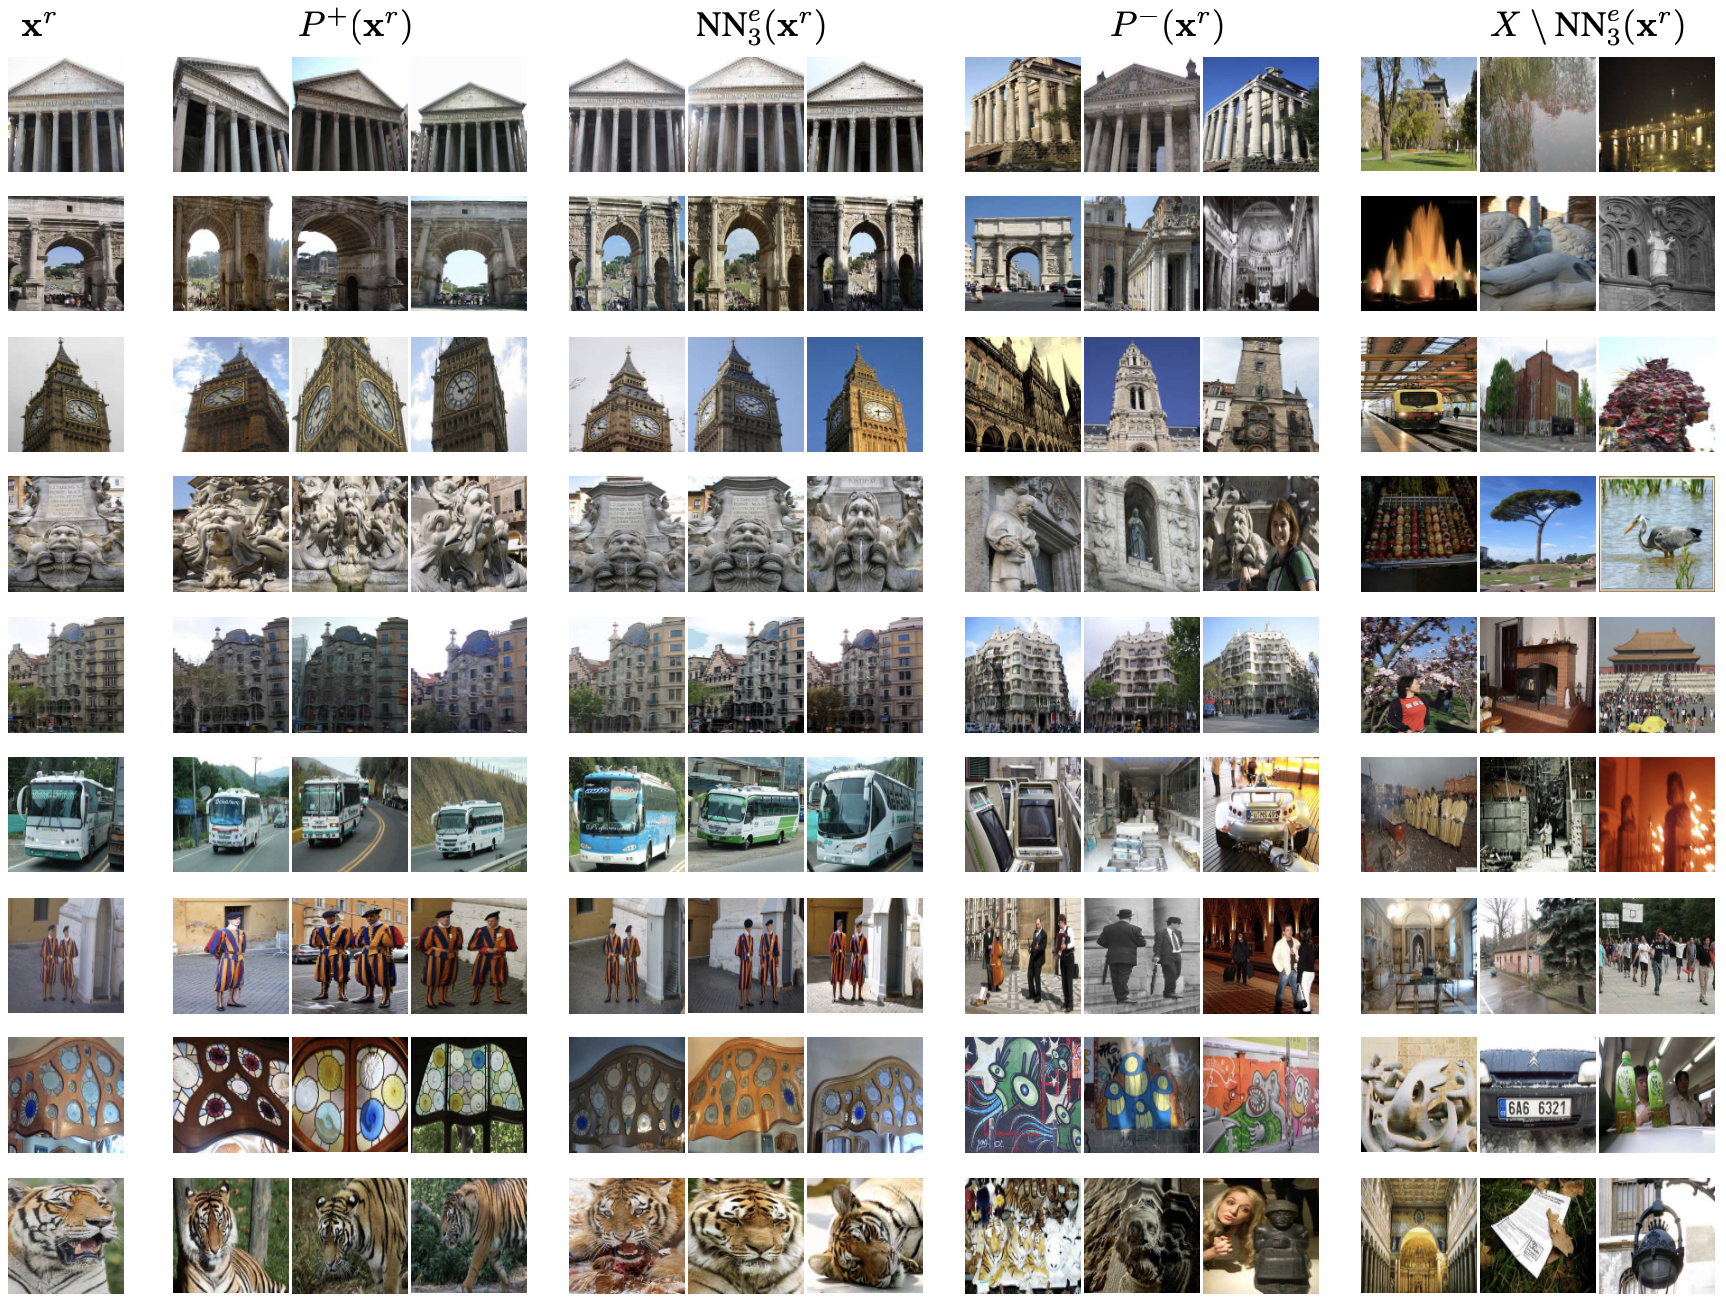
\includegraphics[width=360pt]{images/mining_manifold_examples.png}
    \caption{Illustration Oxford5k and Paris6k images crawled from Flickr from \citet{mining_manifolds_2018}.
    The dataset contains multiple images for each landmark building, i.e. class \citet{manifold_dataset}.
    The anchor is denoted $x^r$.
    A selection of hard positives from $P^+(x^r)$ is compared to the 
    baseline approach by sampling from the closest neighbours to $x^r$ in 
    terms of Euclidean distance.
    Analogously, a selection of hard negatives from $P^-(x^r)$ 
    is compared to the baseline $X \textbackslash NN^e_3$, 
    i.e. sampling from the set that contains all samples but the three closest ones in 
    terms of Euclidean distance.
    It becomes apparent that the hard negatives display visually similar but 
    semantically different images to the anchor. % good
    }
    \label{fig:manifold_mining_examples}
\end{figure}